\documentclass[10pt,a4paper,uplatex,dvipdfmx]{ujarticle} 		% for uplatex
%\documentclass[11pt,a4j,dvipdfmx]{jarticle} 					% for platex
\input{pieces/form00_header} % pieces
\input{pieces/kakenhi7} % pieces
\input{pieces/form01_dcpd_header} % pieces
\input{pieces/hook3} % pieces
%#Name: dc
\input{pieces/form03_dcpd_headers} % pieces
\input{pieces/form04_dc_header} % pieces
% ===== Global definitions for the Kakenhi form ======================
%　基本情報
%
%------ 研究課題名  -------------------------------------------
\newcommand{\研究課題名}{打切り超局所台の関手的性質の研究とMorse理論への応用}

%----- 研究機関名と研究代表者の氏名-----------------------
\newcommand{\研究機関名}{北海道大学}
\newcommand{\研究代表者氏名}{大柴寿浩}
\newcommand{\me}{\underline{\underline{T.~Oshiba}}} 
\input{pieces/inst_general_images} % pieces
% user07_header
% ===== my favorite packages ====================================
% ここに、自分の使いたいパッケージを宣言して下さい。
\usepackage{wrapfig}
\usepackage{amsfonts}
\usepackage{amsmath}
\usepackage[psamsfonts]{amssymb}
\usepackage{amsthm}
\usepackage{mathrsfs}
\usepackage{booktabs}

%\usepackage{amssymb}
%\usepackage{mb}
%\DeclareGraphicsRule{.tif}{png}{.png}{`convert #1 `dirname #1`/`basename #1 .tif`.png}
\usepackage{lineno}
\usepackage{color}
\usepackage{xcolor}
\definecolor{darkgreen}{rgb}{0,0.45,0} 
\definecolor{darkred}{rgb}{0.90,0,0}
\definecolor{darkblue}{rgb}{0,0,0.6} 
\usepackage{enumerate}

% ===== my personal definitions ==================================
% ここに、自分のよく使う記号などを定義して下さい。
\newcommand{\klpionn}{K_L \to \pi^0 \nu \overline{\nu}}
\newcommand{\kppipnn}{K^+ \to \pi^+ \nu \overline{\nu}}
\newcommand{\ctext}[1]{\raise0.2ex\hbox{\textcircled{\scriptsize{#1}}}}

\newcommand{\HOM}{\mathop{\mathcal{H}\hspace{-2pt}om}\nolimits}%内部Hom
\newcommand{\RHOM}{\mathop{\mathrm{R}\hspace{-1.5pt}\HOM}\nolimits}

% ----- 業績リスト用 -------------
\newcommand{\paper}[6]{%
	% paper{title}{authors}{journal}{vol}{pages}{year}
	\item ``#1'', #2, #3 {\bf #4}, #5 (#6).			% お好みに合わせて変えてください。
}

\newcommand{\etal}{\textit{et al.\ }}
\newcommand{\ca}[1]{*#1}	% corresponding author;   \ca{\yukawa}  みたいにして使う
\newcommand{\invitedtalk}{招待講演}

\newcommand{\yukawa}{H.~Yukawa}					% no underline
%\newcommand{\yukawa}{\underline{\underline{H.~Yukawa}}}	% with 2 underlines
\newcommand{\tomonaga}{S.~Tomonaga}

\newcommand{\prl}{Phys.\ Rev.\ Lett.\ }		% よく使う雑誌も定義すると楽

% ===== 欄外メモ ==================
\newcommand{\memo}[1]{\marginpar{#1}}
%\renewcommand{\memo}[1]{}	% 全てのメモを表示させないようにするには、行頭の"%"を消す

%\input{../../sample/simple/contents}	% skip
\input{pieces/hook5} % pieces

\begin{document}
\input{pieces/hook7} % pieces
%#Split: 01_background  
%#PieceName: p01_background
\input{pieces/p01_background_00}
\section{研究の概要と位置づけ}
%　　　　＜＜最大　1ページ＞＞

%s03_abst_background
\noindent
\underline{\textbf{研究課題名：\研究課題名}}
%begin 研究科題名及び研究の概要 ＝＝＝＝＝＝＝＝＝＝＝＝＝＝＝＝＝＝＝＝
%研究課題名：打切り超局所台を用いた層理論の研究
%\textbf{【研究の概要】}
\vspace{-10pt}
\paragraph{【研究の概要】}
多様体\(M\)上の層の複体\(F\)に対し，
\textcolor{darkred}{\textbf{超局所台}}\(\mathrm{SS}(F)\)という，
余接束\(T^{\ast}M\)の部分集合が定義される．
一般に，層の複体に対してその超局所台を調べても
各コホモロジー群の特異方向は分からない．
しかし，
%さらに，
%超局所台を精密化した
\textcolor{darkred}{\textbf{打切り超局所台}}\(
	\mathrm{SS}_{k}(F)
\)を用いるとそれが分かる．
%各次数のコホモロジーに関する議論ができる．
これは例えば，
境界値問題の解の一意性のような，
\(0\)次コホモロジーのみに対してしか成りたたない解析的問題に対し有効である．
%ここで一般に\(\mathrm{SS}_{k}(F)\subset\mathrm{SS}(F)\)がなりたつ．
本研究では
%この打切り超局所台に関して，
%次の2点
%2つを目標に研究
%を行う．
%具体的には，
第1に，
この観点を
%打切り超局所台を用いて，
\textcolor{darkred}{\textbf{層係数Morse理論を応用}}する．
%ことを目指す．
%\cite{ST92}により，Morse理論は層係数に一般化された．
%そこ
層係数Morse理論
では，
%普通のMorse理論での，
関数の臨界点に関する条件が，
超局所台を用いた
%て述べられる
%条件
ものに置き換わる．
%その条件
%そこで，
それを
%さらに
打切り超局所台
%によるもの
に取り替えることで，
%得られる結果も精密化できることが期待される．
%その意味で，
層係数Morse理論を精密化する
ことを第1の目標とする．
%のが目標の一つである．
第2に，\textcolor{darkred}{\textbf{打切り超局所台の一般論を拡充する}}．
まず，打切り超局所台の関手的性質
に関して，
%として
%基本的なもの%，
%例えば，順像・逆像・外部テンソル積での振る舞い
%は，
%先行研究
%\cite{KMS03}
%では
%調べられていないもの，
%しかし，
%例えば
%例えば，
Fourier--Sato変換
のような重要だが明らかになっていないものに
%関する振る舞い
関する振る舞いを調べる．
%記述が無いなど，
%打切り超局所台の関手的性質については，
%不十分な部分
%も
%が多い．
また，
%超局所層理論
%的に
%\cite{KS90}
%で定義された
超局所化関手\(\mu_M\)や\(\mu hom\)関手といった，
超局所層理論において重要な
関手を，
打切り超局所台と相性のよい
形に再構成する．%%%%% どんな関手？
%ことも求められる．
%関手を構成し，
%それらの公式集を作ることが応用上も理論的にも求められるが，不十分である．
%そのような一般理論の部分を拡充するのがもう一つの目標である．
%超局所層理論の，
%特異点論・シンプレクティック幾何・\(D\)加群論を含む様々な分野への
%応用が盛んになっている．
本研究の完成時には，
%それら
層理論を応用するにあたって，
%ための
\textcolor{darkred}{
	\textbf{%
		各コホモロジーに関する詳細な情報が得られるようになる}%
		%適用条件の確認がより簡明になる
	%}
}とともに，
\textcolor{darkred}{
	\textbf{超局所解析への応用が得られる}
}ことが期待される．
%end 研究科題名及び研究の概要 ＝＝＝＝＝＝＝＝＝＝＝＝＝＝＝＝＝＝＝＝＝
\vspace{-16pt}
%begin 研究目的や背景などの概要 ＝＝＝＝＝＝＝＝＝＝＝＝＝＝＝＝＝＝＝＝
%\textbf{【当該分野の状況や課題等の背景】}
\paragraph{【当該分野の状況や課題等の背景】}
超局所台は，層を係数とするコホモロジーが，
各点の周りで，
\textcolor{darkred}{\textbf{どの方向に拡張できないかを記述}}する．
その理論は超局所層理論と呼ばれ，
近年，\cite{Nad09,NZ09}や\cite{Tam18}に代表されるように，
\textcolor{darkred}{\textbf{シンプレクティック幾何への応用}}が盛んになってきた．
とりわけ\cite{GKS12}では，層係数Morse理論を効果的に用いて，
シンプレクティック幾何における重要な問題である
Arnoldの分離不能性定理の新しい証明を与えた．
その他にも，\textcolor{darkred}{
	\textbf{\(D\)加群論・特異点論など，様々な分野に応用}
}されている．

他方，柏原--Fernandes--Schapira\cite{KMS03}は，
\(D\)加群の解の伝播の研究を通じて，
打切り超局所台を定義した．
打切り超局所台は層係数コホモロジーのうち，\textcolor{darkred}{
	\textbf{固定した次数\(k\)以下のものが拡張できない方向を記述}
}する．
この意味で，打切り超局所台は超局所台の
精密化である．
\cite{KMS03}では，打切り超局所台
%に関する
%いくつかの性質が成り立つことが示されている．
%例えば，層の外部テンソル積に関する超局所台の振る舞いについて，
%打切り超局所台を用いることで，それまで
%\(\mathrm{SS}(F\boxtimes G)\subset \mathrm{SS}(F)\times\mathrm{SS}(G)\)
%という包含関係しかしめされて
%より細かい情報が得られることが示された．%%%%%%ちゃんと主張を書くべき？
%しかし，
の順像・逆像関手やテンソル積といった関手を適用した際の振る舞い
については示されている．%ものの，
%関手的性質を始め，
しかし，その他の関手についての振る舞いや，
一般的な性質については，重要にもかかわらず調べ尽くされているとは言い難い．
それにも関わらず，2010年代以降に大きな発展は
見られず，\textcolor{darkred}{\textbf{ほとんど手付かず}}の状態にあると言ってよい．

%これに関しては十分に調べられているとは言い難い．
%例えば，超局所Morseの補題は，
%打切り超局所台を用いて精密化することができるが，それは論文になっていない．

%end 研究目的や背景などの概要 ＝＝＝＝＝＝＝＝＝＝＝＝＝＝＝＝＝＝＝＝
\vspace{-16pt}
%begin 本研究の着想に至った経緯など ＝＝＝＝＝＝＝＝＝＝＝＝＝＝＝＝＝＝＝＝
%\textbf{【本研究計画の着想に至った背景】}
\paragraph{【本研究計画の着想に至った背景】}
以上で述べた状況の中で，超局所Morseの補題と呼ばれる，
超局所台を用いて定式化される主張が，
打切り超局所台を用いるとコホモロジーの次数に関する情報も
含む形に精密化できることに気づいた．
これを援用して，\textcolor{darkred}{
	\textbf{超局所層理論における種々の命題が，
	打切り超局所台により改良できる}
}のではないかと思い至った．
また，それを研究する過程でも，
\textcolor{darkred}{\textbf{打切り超局所台に関する一般論の構築が必要}}であると考えるに至った．
%end 本研究の着想に至った経緯など ＝＝＝＝＝＝＝＝＝＝＝＝＝＝＝＝＝＝＝＝

%begin 参考文献 ＝＝＝＝＝＝＝＝＝＝＝＝＝＝＝＝＝＝＝＝＝＝＝＝＝＝＝＝＝
%\vspace{11pt}
\begin{thebibliography}{99}
	{\small
	\vspace{-4pt}	
	\bibitem[KMS03]{KMS03} M.~Kashiwara, T.~M.~Fernandes, 
	P.~Schapira, 
	\textit{Truncated Microsupport and Holomorphic Solutions 
	of \(D\)-modules}, 
	Ann. Scient. \'Ec. Norm. Sup., s\'erie 4, tome 36, 
	pp.583--399, 2003.
	\vspace{-6pt}	
	\bibitem[KS90]{KS90} M. Kashiwara, P. Schapira, \emph{Sheaves on manifolds}, Grundl. math. Wiss., vol. 292, Springer, 1990.
	\vspace{-6pt}
	\bibitem[GKS12]{GKS12} S. Guillermou, M. Kashiwara, P. Schapira, \emph{Sheaf quantization of Hamiltonian isotopies and applications to nondisplaceability problems}, Duke Math. J. 161 (2012), 201--245.
	\vspace{-6pt}
	\bibitem[Nad09]{Nad09} D. Nadler, \emph{Microlocal branes are constructible sheaves}, Selecta Math. 15 (2009), 563--619.
	\vspace{-6pt}
	\bibitem[NZ09]{NZ09} D. Nadler, E. Zaslow, \emph{Constructible sheaves and the Fukaya category}, J. Amer. Math. Soc. 22 (2009), 233--286.
	\vspace{-6pt}
	\bibitem[ST92]{ST92} P.~ Schapira, N.~ Tose, 
    \textit{Morse Inequalities for \(\mathbf{R}\)-constructible Sheaves}, 
    Adv. Math. 93, pp.1--8, 1992. 
	\vspace{-10pt}
	\bibitem[Tam18]{Tam18} D. Tamarkin, \emph{Microlocal condition for non-displaceability}, Springer Proc. Math. Stat., vol. 269, Springer, 2018, 99--223.
	\vspace{-6pt}
	}
\end{thebibliography}
%end 参考文献 ＝＝＝＝＝＝＝＝＝＝＝＝＝＝＝＝＝＝＝＝＝＝＝＝＝＝＝＝＝


\input{pieces/p01_background_01}

%#Split: 02_purpose_plan  
%#PieceName: p02_purpose_plan
\input{pieces/p02_purpose_plan_00}
\section{【２】研究計画（２）研究目的・内容等}
%　　　　＜＜最大　2ページ＞＞
%s02_purpose_plan_dcpd
%\JSPSInstructions		% <-- 留意事項。これは消すか、コメントアウトしてください。
\vspace{-30pt}
%begin 研究目的と研究計画shorter ＝＝＝＝＝＝＝＝＝＝＝＝＝＝＝＝＝＝＝＝
\subsection*{\ctext{1} 研究目的・研究方法・研究内容}
%\vspace{-10pt}
\paragraph{【研究目的】}
本研究の目的は，打切り超局所台の一般理論の確立と，
それによる層係数Morse理論の精密化を図ることである．
\vspace{-10pt}
\paragraph{【研究方法・研究内容】}
まず，\cite{ST92}で展開された層係数Morse理論を精密化する．
次に，打切り超局所台の関手的性質について重要にもかかわらず
明らかになっていない部分を解明する．
最後に，超局所的関手の打切り版を構成し，それらの性質を調べる．
%上記(1)--(3) 
これらを以下の表\ref{tab1}のとおり行う．

%\vspace{-10pt}

\begin{table}[h]
	\vspace{-11pt}
\begin{center}
	\caption{年次計画}
	\label{tab1}
	\begin{tabular}{cc}\toprule
		年度 & 内容 \\\midrule
		2026（1年目）& (1) 層係数Morse理論への応用 \\
		2027（2年目）& (2) 打切り超局所台の関手的性質の解明\\
		2028（3年目）& (3) 超局所的関手の打切り版の構成とその性質の研究\\\bottomrule
	\end{tabular}
\end{center}
\vspace{-44pt}
\end{table}

\subsection*{\ctext{2} どのような計画で，何を，どこまで明らかにしようとするのか}

表\ref{tab1}各項目(1)--(3)を以下のとおり行う．

\vspace{-11pt}
%\noindent
\subparagraph*{(1) 層係数Morse理論への応用}
%\textbf{(1) 層係数Morse理論の精密化}：

\begin{wrapfigure}{r}{8cm}
	\vspace{-44pt}
	\begin{center}
		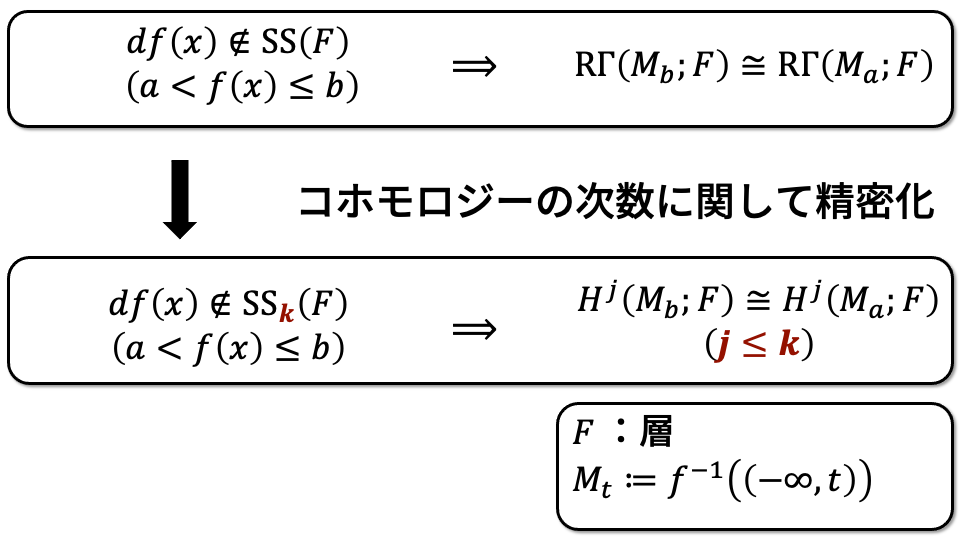
\includegraphics[width=8cm]{figs/dc1-image1.png}
		\caption{層係数Morse理論の精密化}
		\label{fig:image1}
	\end{center}
	\vspace{-22pt}
\end{wrapfigure}

打切り超局所台を用いることで，\textcolor{darkred}{
	\textbf{層係数Morse理論を精密化}
}する．
例えば，\cite{ST92}や\cite{KS90}で
超局所Morseの補題と呼ばれている基本的な命題がある．
この命題の仮定は超局所台を用いて述べられる（図\ref{fig:image1}上段）．
この仮定を打切り\textcolor{darkred}{\textbf{超局所台に取り替えた場合，
結果の部分である導来関手の同型が，
固定した次数\(k\)以下のコホモロジーの同型に
弱まる}}ことを申請者は既に確認している（図\ref{fig:image1}下段）．
そこで，この方向をさらに推し進めて，Morse不等式を精密化する．
\cite{ST92}では，Morse不等式を層係数に一般化するにあたり，
一般の層ではなく，
実構成可能層と呼ばれる特殊な層を考えている．
そこで，本研究でも，\textcolor{darkred}{\textbf{実構成可能層に対する状況設定のもとで．
理論の構築}}を図る．
%ことを目指す．
%(1) の層係数Morse理論について，
%特に，
%ここでは主要な定理であるMorseの不等式を示す．
%\cite{ST92}の設定に基づき，
%実構成可能層を考える．
具体的には，関数を1つ固定し，それと打切り超局所台
から定まる集合を用いて，層係数のBetti数に関する条件を定式化する．
\cite{ST92}では，
大域切断関手の導来関手の各次数の次元に関する不等式として
結果が得られるが，打切り超局所台に取り替えることで，
固定した次数以下の各コホモロジーが（複体でなく）群として現れる．
これらを長完全列等の道具を用いて具体的に計算する．
%属さないことをコホモロジーの同型に言い換える．
%そこから，コホモロジー長完全列等の道具を用いて，
%各次数のコホモロジーの同型を得．
%また，純層や偏屈層と呼ばれるクラスの層（の複体）への応用も目指す．
\vspace{-11pt}
\subparagraph*{(2) 打切り超局所台の関手的性質の解明}
%\noindent
%\textbf{(2) 打切り超局所台の関手的性質の探求}：

	%先行研究\cite{KMS03a,KMS03b}での
	%所謂Grothendieckの六則演算のうち，
	%打切り超局所台の順像・逆像・テンソル積と，
	%法錐に関する性質が述べられている．
	%ところが，
	%内部Hom関手\(\RHOM\)については
先行研究\cite{KMS03}の手法に基づき，
打切り超局所台の関手的性質を調べる．
まず，\textcolor{darkred}{\textbf{Fourier--Sato変換の打切り超局所台について成り立つ
性質}}を求める．
さらに，\cite{KS90}の手法に基づき，
\textcolor{darkred}{\textbf{層がしかるべきコホモロジーに関する条件をみたすとき，
あるいは，多様体の射が，固有的あるいは平滑であるといった状況をみたすとき，
その帰結として得られる他の関手との関係}}について調べる．
とくに，応用上重要な状況である，
射が超局所台に関して非特性的であるという状況を，
射が打切り超局所台に関して非特性的であるという状況に取り替えた場合，
それぞれ得られる帰結を比較する．
\vspace{-15pt}
%\noindent
\subparagraph*{(3) 超局所的関手の打切り版の構成とその性質の研究}
%\textbf{(3) 超局所的関手の打切り版の構成}：
\begin{wrapfigure}{r}{8cm}
	\vspace{-26pt}
	\begin{center}
		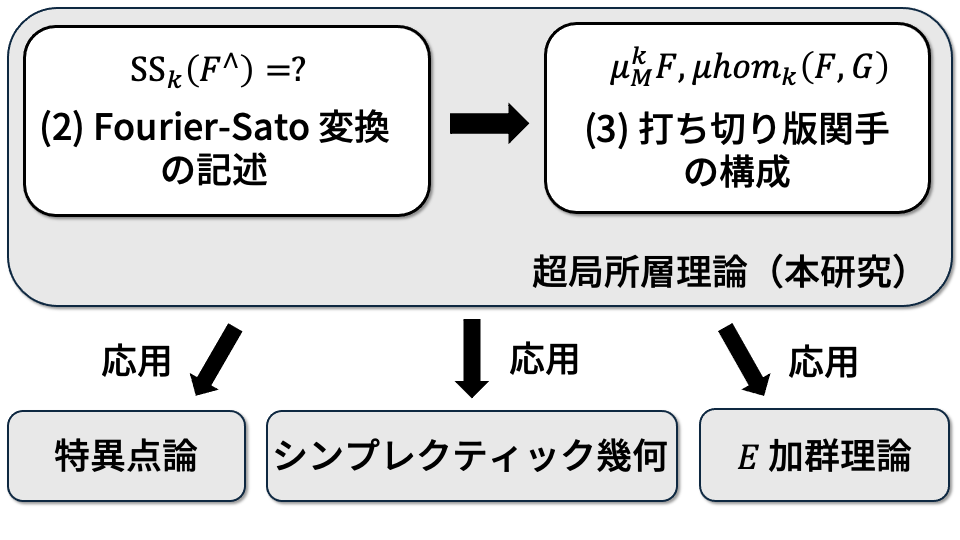
\includegraphics[width=8cm]{figs/dc1-image2-1.png}
		\caption{研究(2), (3) と他分野との関係}
		\label{fig:image2}
	\end{center}
	\vspace{-33pt}
\end{wrapfigure}

\cite{KS90}では，多様体\(M\)上の層\(F\)に対し，
余接束上の層を対応させる超局所化関手\(\mu_M\)や，
その一般化である\(\mu hom\)関手\(\mu hom(F,G)\)が定義されている．
これらをコホモロジーの次数に関して分解した，
\textcolor{darkred}{\textbf{打切り超局所化関手や打切り\(\mu hom\)関手を構成し}}，
その関手的性質を調べる．
超局所化関手はFourier--Sato変換を用いて定義されるが，
(2) でFourier--Sato変換を調べたので，
その性質を用いて打切り版の超局所化も調べる．

%\vspace{-11pt}
%\paragraph*{\ctext{1} 研究目的，研究方法，研究内容}
%\paragraph{【年次計画】}

%\vspace{-10pt}


%\vspace{-20pt}
%\subparagraph{1年目} 
%\vspace{-10pt}
%\subparagraph{2年目}
%2年目は，(2) のとおり，打切り超局所台の関手的性質について調べる．
%とくに，Fourier--Sato変換に関する振る舞いと，
%他の関手との合成が同型になるための条件を
%打切り超局所台を用いて記述する．
%その上で，
%\vspace{-10pt}


%\subparagraph{3年目}
%3年目は，超局所化関手と\(\mu hom\)関手の打切り版を構成し，
%その関手的性質を調べる．
\vspace{-22pt}
\subsection*{\ctext{3} 研究の特色・独創的な点}

%\vspace{-10pt}

\paragraph{【先行研究との比較】}
古典的なMorse理論では，
与えられた2つの実数\(a<b\)の間にMorse関数\(f\)の
臨界値が存在しなければ，
それぞれの劣位集合は微分同相であることが導かれた．
さらにその帰結として定数層係数のコホモロジーの同型が得られた．
超局所台を用いた層係数Morse理論を扱った先行研究\cite{ST92}では，
\(a<f(x)\leq b\)のとき，その微分\(df(x)\)が層の超局所台に含まれなければ，
劣位集合上の大域切断関手の導来関手が同型であることが示された．
この先行研究の状況では，余接束の点が超局所台に含まれるかどうかは，
すべてのコホモロジーが延長可能であるかどうかが判定条件になるので，
各次数のコホモロジーの状況が不明瞭である．
それに対し本研究では，
超局所台を各次数に分解した超局所台を用いるので，
どの次数までコホモロジーが同型になるかという，
\textcolor{darkred}{\textbf{より弱い条件下で精細な情報が得られる}}．

また，先行研究\cite{KMS03a,KMS03b}では，
層の演算に関する打切り超局所台の振る舞いを，
順像・逆像・テンソル積については求めている．
さらに，Whitneyの法錐を用いた打切り超局所台の記述についても求めている．
しかし，Fourier--Sato変換に関する振る舞いや超局所化関手，
\(\mu hom\)関手との関係については
述べられていない．
これに対し本研究では，
以上の\textcolor{darkred}{\textbf{3つの関手と打切り超局所台の関係を与える}}．

また，本研究では，\textcolor{darkred}{\textbf{打切り超局所台という
偏微分方程式論への応用しか考えられていなかった道具
を，層係数Morse理論という幾何に応用}}しようとしている．
それが本研究の独創的な点である．

\vspace{-10pt}
\paragraph{【本研究の完成時に予想されるインパクト】}
上記(1)--(3)について，対応することを述べる．
(1) が完成した場合，層係数Morse理論の応用が一層容易になる．
特に，
この枠組みの元では、\textcolor{darkred}{\textbf{必要とされる条件が特定次数の
%その適用条件が次数の
コホモロジーの延長可能性として明示的に記述できるの}}で，
%導来圏などの手法に不慣れな研究者でも，
%利用することが容易になることが期待される．
%特異点をもつ空間に対するMorse理論への応用が知られているが，
特異点を持つ図形を次数ごとに分解した上で，
各コホモロジーの特異性として定式化すれば，
高次の余次元をもつ特異点論への層係数Morse理論を通した応用がなされうる．

(2), (3) が完成した場合，\textcolor{darkred}{\textbf{特異点論やシンプレクティック幾何，
\(E\)加群理論への，より精細な応用}}が得られる（図\ref{fig:image2}下段）．
例えば，従来の打切り超局所台の理論は\(D\)加群論への応用を見込んで展開された．
本研究では，\(D\)加群の超局所化である\(E\)加群にも適用できる．
そのため，\(E\)加群の解の延長可能性について，
コホモロジーの次数に着目した，
より精密な研究が可能となることが期待される．
その他，本研究により，
境界値問題のような\textcolor{darkred}{\textbf{偏微分方程式論に対しても強力な道具立て}}がなされ，
当該分野の発展に貢献することが期待される．

\vspace{-10pt}
\subsection*{\ctext{4}, \ctext{5}：該当しない}
%\vspace{1cm}
\begin{thebibliography}{99}
		{\small
		\bibitem[KMS03a]{KMS03a} M.~Kashiwara, T.~M.~Fernandes, 
		P.~Schapira, 
		\textit{Truncated Microsupport and Holomorphic Solutions 
		of \(D\)-modules}, 
		Ann. Scient. \'Ec. Norm. Sup., s\'erie 4, tome 36, 
		pp.583--399, 2003.
		\vspace{-6pt}	
		\bibitem[KMS03b]{KMS03b} M.~Kashiwara, T.~M.~Fernandes, 
		P.~Schapira, 
		\textit{Involutivity of Truncated Microsupports}, 
		Bull. Soc. math. France, 131 (2), 2003, 
		pp.259--266.
		\vspace{-6pt}	
		\bibitem[KS90]{KS90} M. Kashiwara, P. Schapira, \emph{Sheaves on manifolds}, Grundl. math. Wiss., vol. 292, Springer, 1990.
		\vspace{-6pt}
		\bibitem[ST92]{ST92} P.~ Schapira, N.~ Tose, 
		\textit{Morse Inequalities for \(\mathbf{R}\)-constructible Sheaves}, 
		Adv. Math. 93, pp.1--8, 1992. 
		%\vspace{-10pt}
		}
\end{thebibliography}
	
%end 研究目的と研究計画shorter ＝＝＝＝＝＝＝＝＝＝＝＝＝＝＝＝＝＝＝＝
\input{pieces/p02_purpose_plan_01}

%#Split: 03_rights  
%#PieceName: p03_rights
\input{pieces/p03_rights_00}
\section{人権の保護及び法令等の遵守への対応}
%　　　　＜＜最大　1ページ＞＞

% s09_rights
%begin 人権の保護及び法令等の遵守への対応 ＝＝＝＝＝＝＝＝＝＝＝＝＝＝＝＝＝＝＝＝
	該当しない．

	%象の卵のES細胞の培養、象のクローンの生成などは行わない。

	%\LaTeX の便利な機能については、\texttt{egg\_***.tex} や\texttt{sample\_pdf/egg\_***.pdf}をご覧ください。
%end 人権の保護及び法令等の遵守への対応 ＝＝＝＝＝＝＝＝＝＝＝＝＝＝＝＝＝＝＝＝

\input{pieces/p03_rights_01}

%#Split: 04_abilities  
%#PieceName: p04_abilities
\input{pieces/p04_abilities_00}
\section{【４】研究遂行力の自己分析}
%　　　　＜＜最大　2ページ＞＞

% s14_abilities
%\SelfReviewInstructions\\% <-- 留意事項：これは消すか、コメントアウトしてください。
%\noindent
%\textbf{(1) 研究に関する自身の強み}\\
\subsection*{(1) 研究に関する自身の強み}
%\PapersInstructions\\ %<-- 留意事項：これは消すか、コメントアウトしてください。
%begin 自己分析 ＝＝＝＝＝＝＝＝＝＝＝＝＝＝＝＝＝＝＝＝
\subsubsection*{研究に対する主体性}
申請者は，文献調査や研究集会，セミナーを通じて，主体的に研究を行っている．
特に，代数解析については学部生の頃から興味をもち，
国際研究集会にも学部生の段階で出席していた．
代数解析の\textcolor{darkred}{\textbf{周辺分野についても，
学外の集中講義や研究集会に積極的に参加}}している．
例えば，シンプレクティック幾何については，
2023年10月に九州大学で行われた集中講義
「層量子化と深谷圏」にはオンラインで参加した．
また，力学系への応用に関して，
2024年9月に熊本大学で行われた「力学系勉強会」には現地で参加した．

その他，申請者は，北大代数解析セミナーや
幾何構造と可積分系セミナーといった学外からの研究者を招待しての
\textcolor{darkred}{\textbf{セミナーに積極的に参加し，幅広い知識を得ることに意欲的}}である．

\subsubsection*{文献調査能力}
申請者の文献調査能力を示す事例として，
本研究の対象である打切り超局所台を知ったきっかけを述べる．
研究室のセミナーで購読している Kashiwara, Schapira, 
\textit{Sheaves on Manifolds} (1990) 
に\(
	\mathrm{SS}(F\boxtimes G)
	\mathbin{\textcolor{darkred}{\mathbf{\subset}}} 
	\mathrm{SS}(F)\times\mathrm{SS}(G)
\)という公式が登場する．
これに対して，
\(D\)加群論での対応物である\(\mathrm{Ch}(\mathcal{M})\)に関しては，
\(
	\mathrm{Ch}(\mathcal{M}\boxtimes \mathcal{N})
	\mathbin{\textcolor{darkred}{\mathbf{=}}} 
	\mathrm{Ch}(\mathcal{M})\times\mathrm{Ch}(\mathcal{N})
\)という公式が成り立つ．記号の意味は説明しないが，
1つ目の公式では片方の包含関係しか示されていないのに対し，
2つ目の公式では等号が成り立つ．
ここで，\(\mathrm{SS}(F)\)に関して逆向きの包含
が成り立つのかどうかを疑問に思った．
周りの専門家に聞いても分からなかったが，
文献を調べていく中で Kashiwara, Fernandes, Schapira, 
\textit{Truncated Microsupport and 
Holomorphic Solutions of \(D\)-modules} (2003) を発見した．
そこでは打切り超局所台の理論を用いて
\(
	\mathrm{SS}(F\boxtimes G)
	\mathbin{\textcolor{darkred}{\mathbf{=}}} 
	\mathrm{SS}(F)\times\mathrm{SS}(G)
\)が示されていた．
これは，\textcolor{darkred}{\textbf{申請者自身がMathSciNetなどのツールを用いて
探し出した}}ものであり，文献調査を通じて自身の疑問が解消できた例である．
以上の事例は，申請者は研究を遂行するために
十分な水準の文献調査能力を有していることを示している．
\subsubsection*{豊富な専門知識と幅広い周辺知識}
申請者は学部1年生の頃から代数解析に興味をもち，前提知識となる
圏論やホモロジー代数，層理論，微分方程式論などを主体的に学習してきた．
大学院に入学してからは，
研究室セミナーでの購読を通じて超局所層理論の基礎的な知識を学習している．
その過程で，重要な補題である非特性変形補題については，
そのアイデアの源泉であるZernerの仏語の原論文
\textit{Domaine d'holomorphie des fonctions v\'erifiant 
une \'equation aux d\'eriv\'ees partielles} 
を通読した上で和訳を作成し，研究室メンバーに共有した．
このように申請者は，\textcolor{darkred}{\textbf{代数解析について，
歴史的な背景や原論文に関する情報を
含む豊富な知識}}を持っている．

また，代数解析の応用として近年盛んになっている
\textcolor{darkred}{\textbf{シンプレクティック幾何を中心に，周辺分野の学習にも積極的}}に取り組んでいる．
今すぐに研究につながるとは限らない知識についても，
上記の文献調査やArXiv・雑誌購読も通じて，
興味のある分野や事実について幅広く知識を身につけるよう心がけている．
\subsubsection*{語学を含む研究上のコミュニケーション能力}
研究集会や研究打ち合わせ等での研究者とコミュニケーションを取ることは，
研究を遂行し，発表する上で欠かせない．
その観点で，申請者は十分なコミュニケーション能力を有している．
例えば，2024年10月に京都大学数理解析研究所で開催された
研究集会「超局所解析と漸近解析の展望」で海外の研究者が講演を行った際，
\textcolor{darkred}{\textbf{英語での質問・議論}}を行い，
後日，指導教員を通して，質問の鋭さに対しての賞賛も頂いた．
また，国内でも，研究集会やセミナーの際に講演者と積極的に議論をしている．
以上のことから，
申請者は研究を遂行する上で十分なコミュニケーション能力を有しているといえる．

\subsubsection*{自主的な課題設定と発想力}
%上記の文献調査を通じて，
上記の文献調査や学内外の研究者とのコミュニケーションを通じて，
申請者は主体的に課題を設定し取り組んでいる．
例えば本研究も自身の発想に基づく．
研究集会やセミナーでも積極的に問題の拡張，応用について考察し，
質問したりしている．

\subsubsection*{プレゼンテーションを含む説明能力}
研究集会やセミナーでの発表では，聴衆の反応を確認しながら，
理解できるよう説明をするのが重要である．
その点申請者は，
聴衆の背景知識の確認・スライドやノートの作成・プレゼンテーション・質疑応答
の各段階において，それぞれ十分な能力を持っている．
例えば，申請者の学部時代の所属サークルである数学研究会では，
定期的に講演会を開催し，
背景知識をあまり持たない低学年の学生向けに少し進んだ数学の講演を行っていた．
そこでの申請者の発表は低学年の学生にも広く受け入れられていたように思う．
実際，そこでの講演をきっかけに興味を持った後輩が，申請者に自主セミナー
を見るよう頼んできたことも複数回あった．

説明能力に関しては，2024年度後期に学部生の位相空間論の\textcolor{darkred}{\textbf{演習のTA}}を担当し，
各回の演習の採点と講評を毎回行った．
そこでの学生から講評だったようで，今学期に引き続き同じ教員の，
今度は基礎的な幾何学の演習授業のTAを任せてもらっている．

以上は，申請者がプレゼンテーションを含む説明能力を有していることを示している．
%end 自己分析 ＝＝＝＝＝＝＝＝＝＝＝＝＝＝＝＝＝＝＝＝

%\vspace{5mm}
%\noindent
%\textbf{(2) 今後研究者として更なる発展のため必要と考えている要素}\\
\subsection*{(2) 今後研究者として更なる発展のため必要と考えている要素}
%begin 今後必要な要素 ＝＝＝＝＝＝＝＝＝＝＝＝＝＝＝＝＝＝＝＝
\subsubsection*{外部の研究者との交流}
本研究の属する超局所層理論は，
必要な知識も応用も広い．
そのため，\textcolor{darkred}{\textbf{国内外を問わず外部の研究者と交流を行うこと}}が重要である．
特に国外においては，フランス・イタリアの研究者が
盛んに超局所層理論を研究している．

北海道は地理的に，他の地域とのやりとりが難しいところもあるが，
\textcolor{darkred}{\textbf{研究集会やセミナーに積極的に参加し，
意見交換をおこなうこと}}が今後の代数解析・超局所層理論の
発展のために重要であると考える．

\subsubsection*{隣接分野の知識}
本研究自体，超局所層理論内部に閉じた部分の研究に重点をおいているものの，
今後の発展を考えると，
\textcolor{darkred}{\textbf{直接の応用となりうる，特異点論・シンプレクティック幾何・偏微分方程式論に
について，より深い知識を身につけること}}が必要と考える．
とくにシンプレクティック幾何においては，超局所層理論を用いた研究のほかに
フレアホモロジーを用いた手法，生成関数を用いた手法，
パーシステントホモロジーを用いた手法がよく知られており，各々の手法の比較や
一つの手法を別の手法に輸入することが近年盛んに行われている．
そのため，これらの分野について，\textcolor{darkred}{\textbf{超局所層理論とのつながりを意識しながら，
研究集会や当分野の研究者との対話を通じて，
主体的に学習することが必要}}であると考えている．

%end 今後必要な要素 ＝＝＝＝＝＝＝＝＝＝＝＝＝＝＝＝＝＝＝＝

\input{pieces/p04_abilities_01}

%#Split: 99_tail
\input{pieces/hook9} % pieces
\end{document}

